% !TEX root = ../../thesis.tex

% \cleardoublepage
% \newpage
% \thispagestyle{plain}
% \mbox{}
% \includepdf{/Users/matthieulapeyre/Documents/phd_thesis/media/thebeast.pdf}
\chapter{Robot morphology: some facinating work} % (fold)

\cleanchapterquote{The world is its own best model}{Brooks}



\section{The emergence of embodiement} % (fold)

EmbedIT – An Open Robotic Kit for Education
\url{http://www.eucognition.org/index.php?page=tutorials}

Since the introduction of numerical computers in the robotic field, research on artificial intelligence has been more and more detached from the actual robot body (Chapuis, Droz, 1949).
The robotic community is then divided into 2 complementary fields.
The artificial intelligence term was introduced in a workshop organized in 1956 by a MIT professor John McCarthy. Globally participant were convinced that by using the notion of computation or abstract symbol manipulation it would be possible to reproduce interesting abilities similar to human ones (McCorduck's Machins who think, 1979) (Haugeland, 1985) . The symbol-processing paradigm or cognitivistic paradigm see the cognition as pure computation. In other word, the relevant intelligence process is the abstract algorithm or the program. Eventually, researchers following this paradigm no longer saw the physical incarnation as a relevant component.
Cognitive and computationalists hypotheses stating that the thought is reducible to a set of symbolic calculations are being etablished (Fodor, 1987). The body, for its part, is forgotten, irreparably separated the mechanisms of intelligence \cite{kaplan2008corps}.
While a research field is focused on exploring intelligence without body, the other one is building body without intelligence, interested in the way to create better actuator or sensors, more precise and powerful. These robots became able to produce high precision task in manufacture but require perfectly controlled and predictable environment. Going outside this known environment seems impossible to program.


In the end of 80's, a novel thought emerged thanks to researchers such as Rodney Brooks~\cite{brooks1991intelligence}, Luc Steels~\cite{steels1995artificial} or Rolf Pfeifer~\cite{pfeifer2001understanding}. In particular, the embodied artificial intelligence rejects the symbolic approach and postulates that it is not possible to have intelligence without the body and the environment~\cite{pfeifer2001understanding}. In this new paradigm the cognition needs a body to think. Even for mathematical thinking we could assume is purely abstract (Lakoff and Nunez).
Rather than postulating there is a hierarchical structure in which the brain control the body, the new theory focuses on the interaction between the two systems.

Classical approach known great successes to solve abstract problem such as chess game, search engine, text processing, however it failed in the understanding of natural forms of intelligence which requires a direct interaction with the real world. This is especially the case when we think in the current state of the art for interaction with human (natural langage) or object (grapsing) and the locomotion in an open environment (walk,
run, ride a bicycle).

The locomotion is a great example of task where the classical robotic approaches globally failed. Animals are incredibly skilled, even if we take insect with a brain thousand of times smaller than the human one, their abilities to move in an open world is just incomparable with the most advanced current robot.

One important reasons for this is that in the classical view, the ability to figure out where you are is based in detailed inner models or representaiotns either have to be programmed into the robots or learn by interacting with the environnement and continously updated. The more complex these models are, the more effort is needed to accquire the relevant data to maintain them leading to major problem when learning task in a high dimensionnal space (plein de ref).

Brooks argued in (1991a) that intelligence always requires a body and that we should forget about complex internal representaitons and models of hte outside world; that we should not focus on sophisticated reasoning processes but rather capitalizer on the system-environment interation. Then he started to work on the insect locomotion () because if we understand the insect-level-intelligenec it will be much easier and faster to understand and build human-level intelligence.

Thus an interesting evolution of the last decades is the demonstration of the importance of the morphology for sensorimotor control, cognition and development.

Les « tortues » cybernetiques de Grey Walter construites en 1948 sont alors prises comme exemple de ce que doit etre une bonne conception integrant de maniere fine la conception de la machine physique aux comportements souhaites. Ces robots entierement analogiques etaient capables de comportements complexes, sans pour autant utiliser de « representations » internes (Guy Walter, 1949). Leur conception tenait compte du fait qu’il s’agissait de machines physiques, soumises a la gravite ou aux frictions, qui produisent leur simulation sensorielle par leur propre mouvement. La nature et la disposition de leur systeme sensoriel leur permettaient de resoudre des « taches » complexes comme retrouver leur station de recharge, sans qu’il soit necessaire pour autant de faire appel a un quelconque « raisonnement ».
The role of the morphology appears as a fascinating open field. Exploring the interaction between body properties and cognition could lead to both a better understanding of animals’ behaviour (human being in particular) and to build robot more adapted and robust to an open environment with unpredictable interaction. In particular we can highlight the acquisition of sensorimotor task and the exploration of adapted bodies for natural physical and social interaction with humans.

In this context, we should not only take care of the robot body design but both introduce the morphology as an experimental variable and conduct experiments in the real world, indeed \emph{the best model of the world is the world itself} - Rodney Brooks~\cite{brooks1991intelligence}.

\begin{figure}[]
    \centering
    \begin{boxedminipage}{0.95\textwidth}
        \textbf{Mechanical calculus}\\
        Once upon a time, in a age transistors were not here, complex calculus was done using mechanical properties.
        Using complex mechanisms the very first calculators were fully mechanical machine (see \figurename~\ref{fig:mechanical_computer}).

        The first freely programmable, binary, floating-point, general-purpose mechanical computer in the world was the Z1 constructed by Zuse between 1936 and 1938 (see \figurename~\ref{fig:zuse_z1}).
        This "computer" contained approximately 30,000 components and was incredibly sophisticated, making the Z1 suitable for a wide variety of engineering and scientific applications.
        Introduced by Curt Herzstark in 1948, the Curta (see \figurename~\ref{fig:curta_calculator}) is a small, hand-cranked digital mechanical calculator.
        It can be used to perform addition, subtraction, multiplication, division, and (with more difficulty) square roots and other operations.
        The Curta's design is a descendant of Gottfried Leibniz's Stepped Reckoner and Thomas's Arithmometer, accumulating values on cogs, which are added or complemented by a stepped drum mechanism.
        It has an extremely compact design: a small cylinder that fits in the palm of the hand.

        These two examples show that even pure calculus is acheivable using only morphological properties (here mechanical) and was used during dozens of years for scientific applications.


        Curtas were considered the best portable calculators available until they were displaced by electronic calculators in the 1970s.

        \begin{center}

            \subfloat[][Zuse Z1 (1936)]{\label{fig:zuse_z1}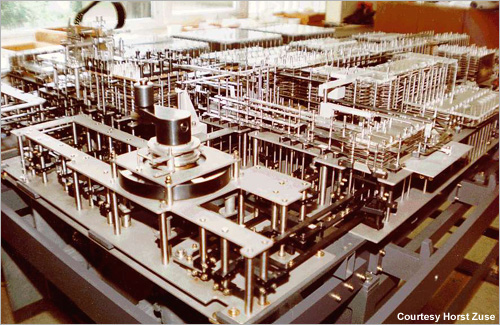
\includegraphics[width=0.42\linewidth]{hist-z1-reconstruct.jpg}}
            \hfil
            \subfloat[][Curta]{\label{fig:curta_calculator}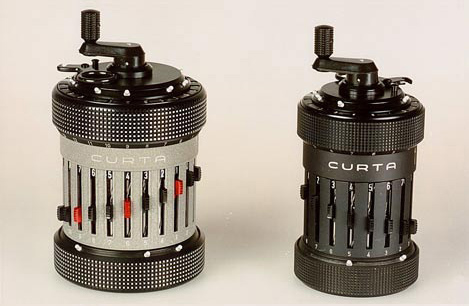
\includegraphics[width=0.42\linewidth]{curta_calculator.jpg}}
            \caption{Mechanical calculus machines}
            \label{fig:mechanical_computer}

        \end{center}

    \end{boxedminipage}
\end{figure}

\section{Morphological computation} % (fold)

intro qu'est ce que le morphological computation.

% Indeed, while for decades "think is calculate" leading to complex robot needed huge computation power to explicitely compute dynamics and complex stuffs. However, while we can indeed sugest that there are calculus in the way we move, this calculus can be implicit. Morphological properties can

\subsection{The fly} % (fold)

To go futher in the understanding of the emboiement intelligence, we

For decades (and it is still the case) roboticists try to solve the locomotion, in particular the biped one with complex behavior based on high-speed full dynamics calculus of internal model. But if being able to move was only a question of intelligence, flying should note be a problem for us. We are way more intelligent than a fly, we should be able to it easily !

Anyone saying that will look kind of idiot in front of its audience, no ? However, given the current robotiscist approach, it is somehow logical. If being able to act in the environnement was only an computational problem, then anyone more intelligent, meaning able to perform more calculus, than a flying creature should be able to fly.

Of course, it does not make any sense and we understand easily why. Even a really intelligent creature needs a body to actually fly. With our currently biased point of view it would be even difficult to imagine a flying creature whitout proper wings.

More than that, the actual achievement of the fly does not require any computation. Everything needed is described by the nature law expressed by Bernouilli and an adapted morphology. It is pure morphological computation and it allows to achieve a locomotion as complex as the fly !



Make a machine fly is one the great scientific and engeenering example acheived thanks to a deep understanding of the interaction between the environnement and the morphology.

Indeed a plane has to deal with its environnement which is the "air".

While ones could see the real air as a constraint because of its viscousness and prefer model it as a perfect fluid in simulation, it would be impossible or at least way more complicated to make a plane fly. Indeed, it is because the air is viscous that the fly is possible.

Actually a plane fly only thanks to the interaction between its specific wing morphology and the environnment fluid which is the "air".

\begin{equation}
    F_{lift} = \frac12 \times \rho \times V^2\times S \times C_z
\end{equation}

To create lift, the only variable are the profil shape which give the $C_z$ parameter and the surface voilure $S$ and the air properties with its volumic mass $\rho$ and the velocity of the flux $V$.

\begin{equation}
    adapted morphology + air = fly
\end{equation}

If we look like to another complex bevahior such as the fly. With this approach we could think the fly need a large amount of explicit calculus. However the aeronautic people already understand that the plan they are trying to make fly will act in the real world and the real world is the "air". A plane can only fly because of the air and because it is viscous. The air is not a constraints it is the central element for make a plane fly.

All the intelliegence is centered around the wing shape.


Another great example of how mechanics properties can produce complex behavior is the airplane.
The lift force generated by wings are the resulting of the interaction between a air flux and the physical profil shape of the wing.
Then the Bernouilli law add the necessary magic around to make plane fly (see \figurename~\ref{fig:magic_plane})

we can change the behavior by hanging the wing shape, some fighter have a voilure variable

To resume, a plane can work thanks to the fact the air is not a perfect fluid and because it has an adapted morphology. Even rocket use aerodynamic to improve the stability otherwise it would be really complex to keep a direction.



The only way to make machine "fly" without these specificities is to create a rocket which need a very high power to oppose the gravity and complex control to

\begin{figure}[tb]
    \begin{center}
        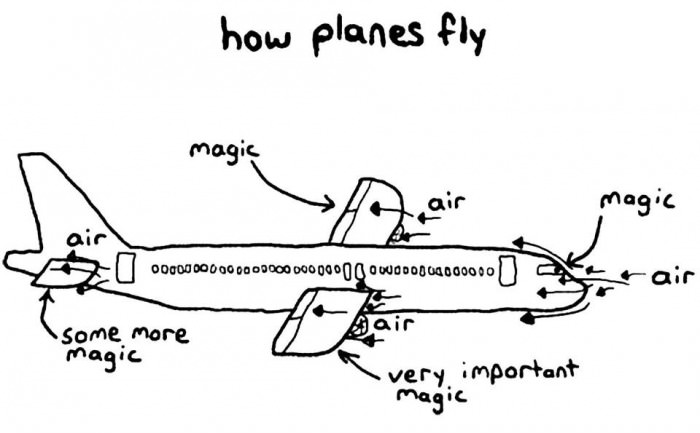
\includegraphics[width=0.8\linewidth]{plane_explanation.jpg}
    \end{center}
    \caption{Caption here}
    \label{fig:magic_plane}
\end{figure}

\begin{figure}[]
\centering
    \subfloat[][]{\label{}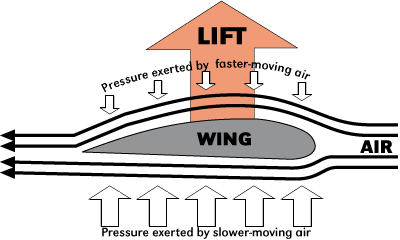
\includegraphics[width=0.56\linewidth]{bernoulli_wing_lift.png}}
    \hfil
    \subfloat[][]{\label{}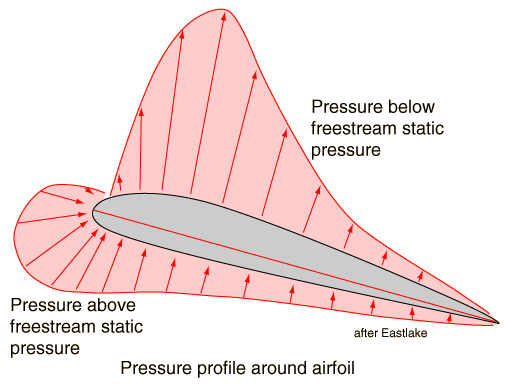
\includegraphics[width=0.42\linewidth]{airfoil_bernouilli.png}}
    \caption{}
    \label{fig:}
\end{figure}

After 60 years of fly history with hundreds of actual plane from planneur to airbus A380, it looks obvious that the shape of the plane is a major, or event the most important part. However, then discussing of legged locomotion, from centipedes to biped ones, the question of the morphology is often left aside in favor to computationnal model. Is there really a fundamental reason the body should be irrelevant for legged locomotion while being essential for flying? There is a lot of legged animals and they are not smater than the flying or swimming ones. Is there a fundamental law comparable to the Bernouilli one ? It can be a biological, a mechanical or even a chimical law, yet it deserves to be explored.

While the velocity of legged locomotion are in most of the case quite low, we could ignore air friction, then a first track could be the interaction between the newton's law and the ground. Using gravity as an advantage instead of a force we have to battle.

This set-up the work of Tad McGeer, comming from the aeronautic field, he was surprised by how the actual legged robot morphology was neglected. A great example is the Tad McGeer's passive walker. Thanks to the understanding of the intrinsic dynamics of its structure, Tad McGeer has managed to create a 2D biped robot capable of producing several steps without any controller or motor showing that such a complex task can be indeed achieved only with adapted morphology\cite{mcgeer1990passive}.

The result is comparable to the sailplane or the paper plane. Using a specific mass repartition and foot shape interecting with gravity and the ground ...

The role of morphology in robot biped locomotion has been particularly explored through the research on passive dynamic walkers~\cite{wisse2007passive}.
The most famous example concerns the Tad MacGeer's work~\cite{mcgeer1990passive}.
Thanks to the understanding of the intrinsic dynamics of its structure, McGeer has managed to create a 2D biped robot capable of producing several steps without any controller or motor.
The only control of this robot is obtained through the interaction between the intrinsic inertia of the structure and gravity.

\begin{figure}[]
\centering
    \subfloat[][Tad McGeer with his prototypes]{\label{fig:tad_mcgeer}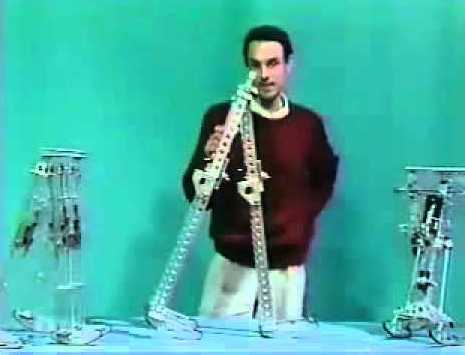
\includegraphics[width=0.49\linewidth]{tad_mcgeer.jpg}}
    \hfil
    \subfloat[][Passive walker robot]{\label{fig:mcgeer_walker}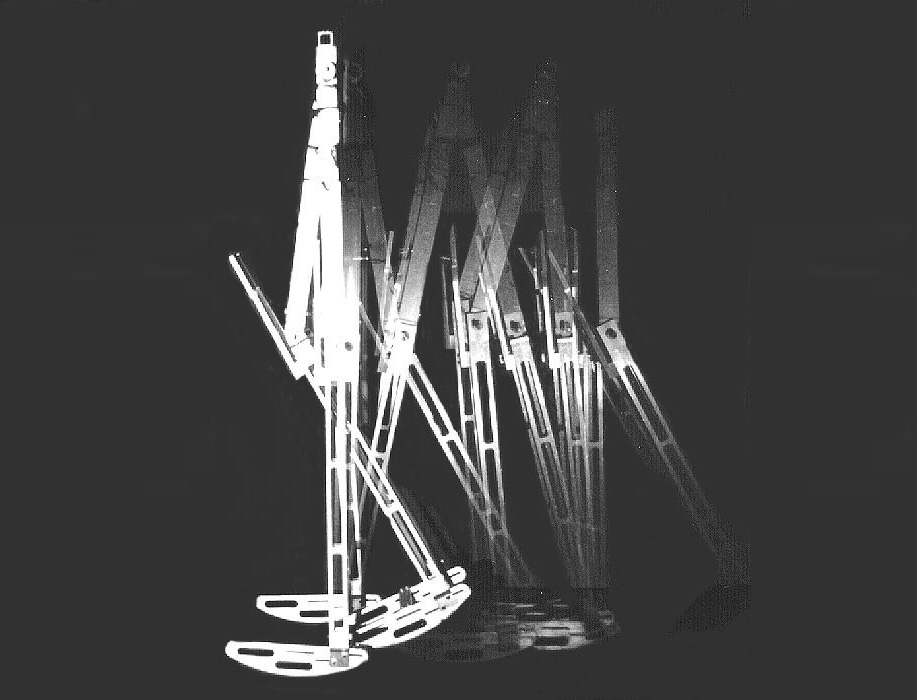
\includegraphics[width=0.49\linewidth]{mcgeer_walker.jpg}}
    \caption{}
    \label{fig:mcgeer_work}
\end{figure}

This work has been pursued with the apparition of semi-passive walker combining both specific passive properties and low power actuation to increase their robustness~\cite{Anderson2005}.
We can note the work of Collins~\cite{collins2005bipedal} which explored the case of semi-passive 3D biped robot.
Its morphology is based on particular mass distribution, knee locking, round feet and springs on the legs to generate an efficient walking gait while keeping its lateral and frontal balance.
The concept of 3D semi-passive robot has been pushed even further with the realization of a complete humanoid robot with trunk, arms and head: the robot Denise~\cite{wisse2005three} and Flame presented in~\cite{Hobbelen2008}.

http://tensegritywiki.blogspot.fr/2010/08/mechanism-as-mind-tensegrity-and.html




\section{Exploration de la morphologie dans la robotique} % (fold)


\section{Robotic} % (fold)
For years, artificial intelligence was only considered through complex computation.
An interesting evolution during the last decade was the emergence of work showing the importance of the actual robot morphology in the robot behavior.

The concept of morphological computation has also been associated to the principle of “ecological balance”, as outlined by Pfeifer et al.
\cite{pfeifer2005new}, which states that there is a balance or task distribution between morphology, materials, control, and interaction with the environment.
For example, morphological computation has been shown to be necessary in order to achieve human-like biped locomotion \cite{matsushita2005locomoting} and the coupling of adequate morphologies with central-pattern generators has been shown to generate robust locomotor behavior \cite{ijspeert2007swimming}\cite{steingrube2010self}.


It has also been shown that the compliance of the body explains the dynamics of walking and running \cite{Geyer2006} and several biped robots such as Athlete Robot \cite{niiyama2010athlete} or BioBiped1 \cite{radkhah2011concept} were designed using compliant actuator or elastic material.
These robots showed interesting hopping and running behavior while using less power actuator than common humanoid robot such as Asimo or HRP-2.

Among all robots designed to explore morphological computation and compliant body only few allow to explore physical interaction such as Kenshiro \cite{Asano2012} or Acroban which the compliant structure of its vertebral column and legs was shown to permit a self-organized physical human-robot interface allowing non-expert users to lead the robot by the hand \cite{Ly2011bio}\cite{Oudeyer2011}.

The morphological properties of these robotic platforms are especially interesting but unfortunately they are difficult and expensive to reproduce by other research laboratories.
Most of the studies made on the humanoid robot locomotion in the past 30 years~\cite{park1998biped}~\cite{aoi2005locomotion}~\cite{park1998biped} mainly focus on tackling the challenge of biped walking through the active control of the whole robot dynamics using technics such as ZMP control~\cite{vukobratovic2004zero} requiring very precise and high torque actuation~\cite{akachi2005development}.

The properties of the robot morphology have shown interesting results for robust locomotion, for instance the hexapod robot Rhex~\cite{saranli2001rhex}.
Still, it is surprising that only few explored the challenge of biped locomotion through the study of the role of morphology.
One can cite the work of Chandana Paul and Josh C.Bongard~\cite{paul2001road} and Ken Endo~\cite{endo2002co} which have explored evolutionary optimization on robot morphology to achieve stable biped locomotion.
They have showed a strong impact of the morphology on the walking behavior and were able to reduce the complexity of the controller by finding good mechanical properties (limbs length and mass distribution).
It has also been shown that human morphological properties such as the compliance of the body explains the dynamics of walking and running \cite{Geyer2006} while experiments made by Kojiro Matsushita~\cite{matsushita2005locomoting} show that an adequate morphology is needed if one is interested in natural looking kind of locomotion.




Several studies have also explored the role of the foot and ankle morphology for biped walking on both human~\cite{Adamczyk2006}~\cite{Hughes1990} and robot~\cite{hobbelen2005ankle}~\cite{Davis2010}.
However, to our best knowledge no research has focused on the role of the thigh for biped locomotion.
While the HRP-4C~\cite{kaneko2009cybernetic} and Kenshiro humanoid~\cite{nakanishi2013design} robot seem to visually have a morphology design close to the thigh shape of Poppy, they did not study, in the associated scientific papers the role of this shape on the dynamic of their humanoid robot.
Most of the studies made on the humanoid robot locomotion in the past 30 years~\cite{park1998biped}~\cite{aoi2005locomotion}~\cite{park1998biped} mainly focus on tackling the challenge of biped walking through the active control of the whole robot dynamics using technics such as ZMP control~\cite{vukobratovic2004zero} requiring very precise and high torque actuation~\cite{akachi2005development}.

Regarding the role of morphology in biped locomotion, one of the first famous example concerns the work of Tad MacGeer on passive dynamic walkers \cite{mcgeer1990passive}.
Thanks to the understanding of the intrinsic dynamics of its structure, McGeer has managed to create a 2D biped robot capable of producing several steps without any controller or motor.
The only control of this robot is due to the interaction between the intrinsic inertia of the structure and gravity.
This work has been pursued by those of Collins \cite{collins2001three} and Tedrake \cite{Tedrake2004}  who perfected the concept to make 3D walkers possible and over longer distances.
The structure of its robot has its own dynamic that allow it to self-stabilize and maintain a walking motion.



\subsection{Passive dynamic walkers} % (fold)



\begin{figure}[]
    \begin{center}
        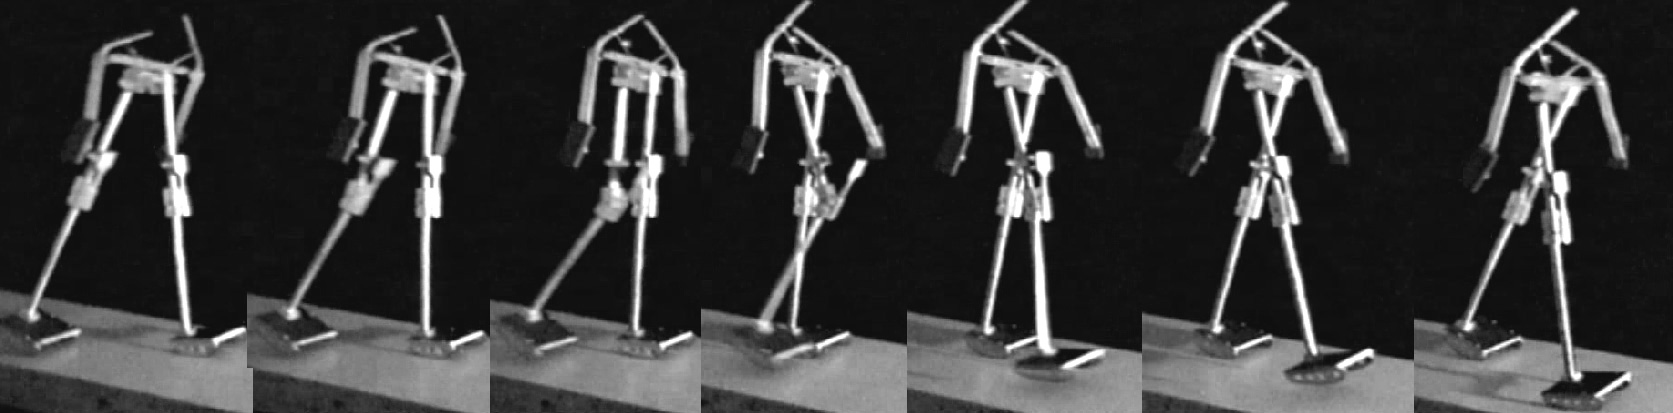
\includegraphics[width=0.99\linewidth]{cornell_biped_series.jpg}
    \end{center}
    \caption{Caption here}
    \label{fig:figure1}
\end{figure}

\begin{figure}[]
    \begin{center}
        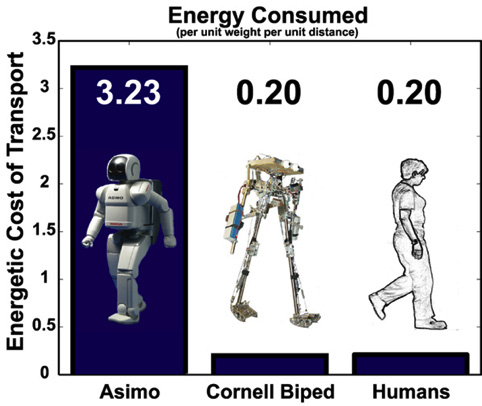
\includegraphics[width=0.6\linewidth]{comparison_cost_transport.jpg}
    \end{center}
    \caption{Caption here}
    \label{fig:figure1}
\end{figure}



\section{Complex emergent behavior} % (fold)


\begin{figure}[]
\centering
    \subfloat[][]{\label{}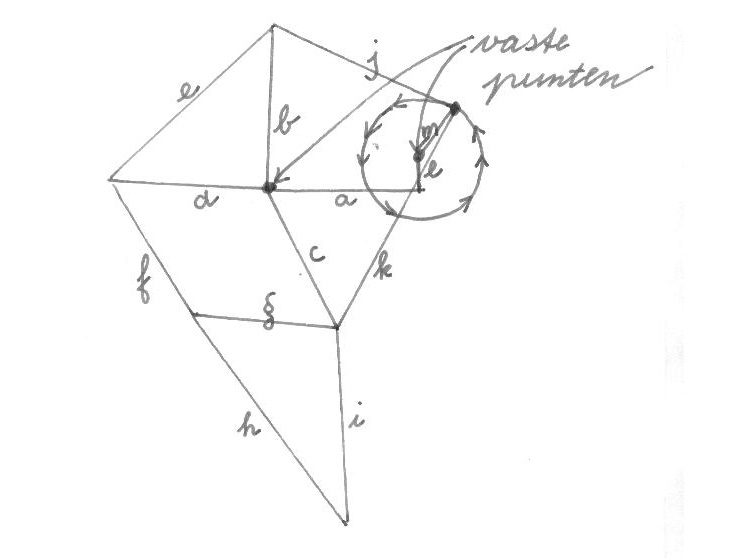
\includegraphics[width=0.32\linewidth]{strandbeest_theory.jpg}}
    \hfil
    \subfloat[][]{\label{}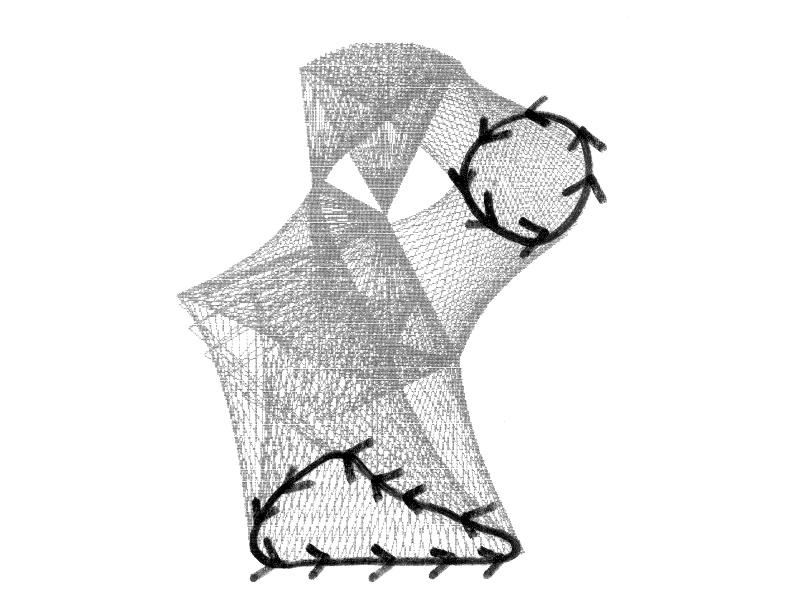
\includegraphics[width=0.32\linewidth]{strandbeest_motion.jpg}}
    \hfil
    \subfloat[][]{\label{}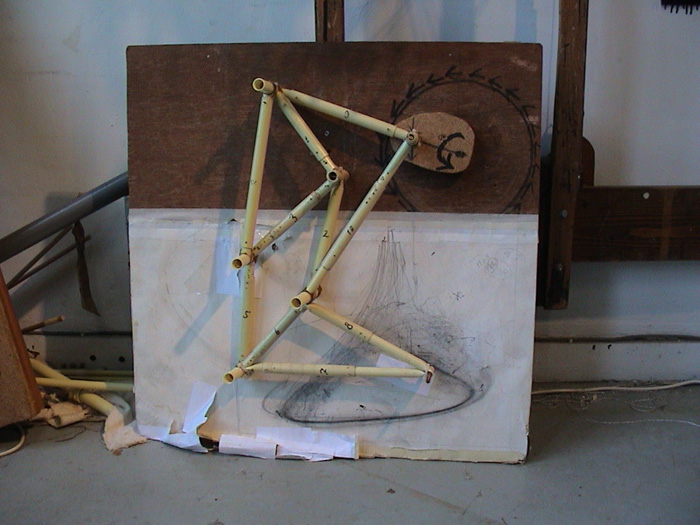
\includegraphics[width=0.32\linewidth]{strandbeest_leg_element.jpg}}
    \caption{}
    \label{fig:}
\end{figure}


\begin{figure}[]
    \begin{center}
        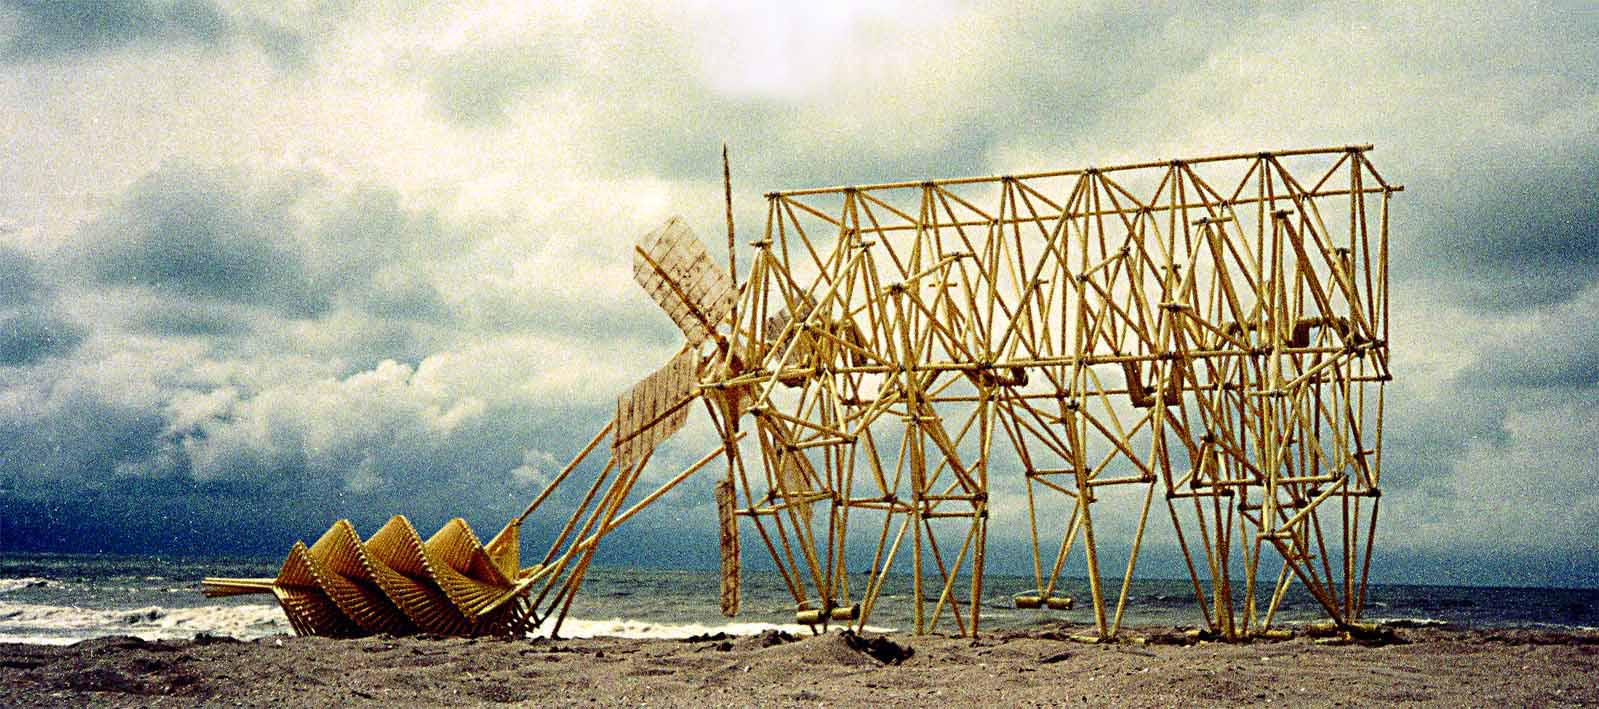
\includegraphics[width=0.99\linewidth]{theo_jansen_beast.jpg}
    \end{center}
    \caption{Caption here}
    \label{fig:figure1}
\end{figure}



\section{Morphology as an experimental variable} % (fold)
\label{sec:morphology_as_an_experimental_variable}

% section morphology_as_an_experimental_variable (end)


\subsection{Locomotion} % (fold)

\subsection{Robustness} % (fold)


\section{Morphology and cognition} % (fold)

\subsection{Data filter} % (fold)

exemple de l'oreille

\subsection{Control stuff} % (fold)

La compliance c'est chouette


Scientific study of the role of morphology in sensorimotor control and cognition: in Robotics (McGeer, Pfeifer and co.), in relation with Cognitive Science (e.g.
http://www.pyoudeyer.com/IEEETAMDOudeyer10.pdf ) and animals (e.g.
work of Robert Full)

\textbf{Object}: In this chapter, we will present a review of different research which has already explored the role of the mophology


\textbf{Conclusion}: The body can definitely take in charge a part of the complexity.
And we need to continue studying it by EXPERIMENTATIONS.
Even if simulator can be complementary.
% chapter exploration_of_the_morphology_role (end)

